\documentclass{gescons}

\genre {Entrevista}
\author{Ricardo Rezende}
\title{Autoidentificação Proexológica}
\paginaurl{https://www.youtube.com/live/GY1e0RQYrtg}

\begin{document}
    \makeentrevistatitle
    \coverart{back/Ricardo_Rezende_Autoidentificao}

    \begin{multicols}{2}


%\noindent\includegraphics[width=9cm, height=10cm]{example-image} 
\begin{center}
    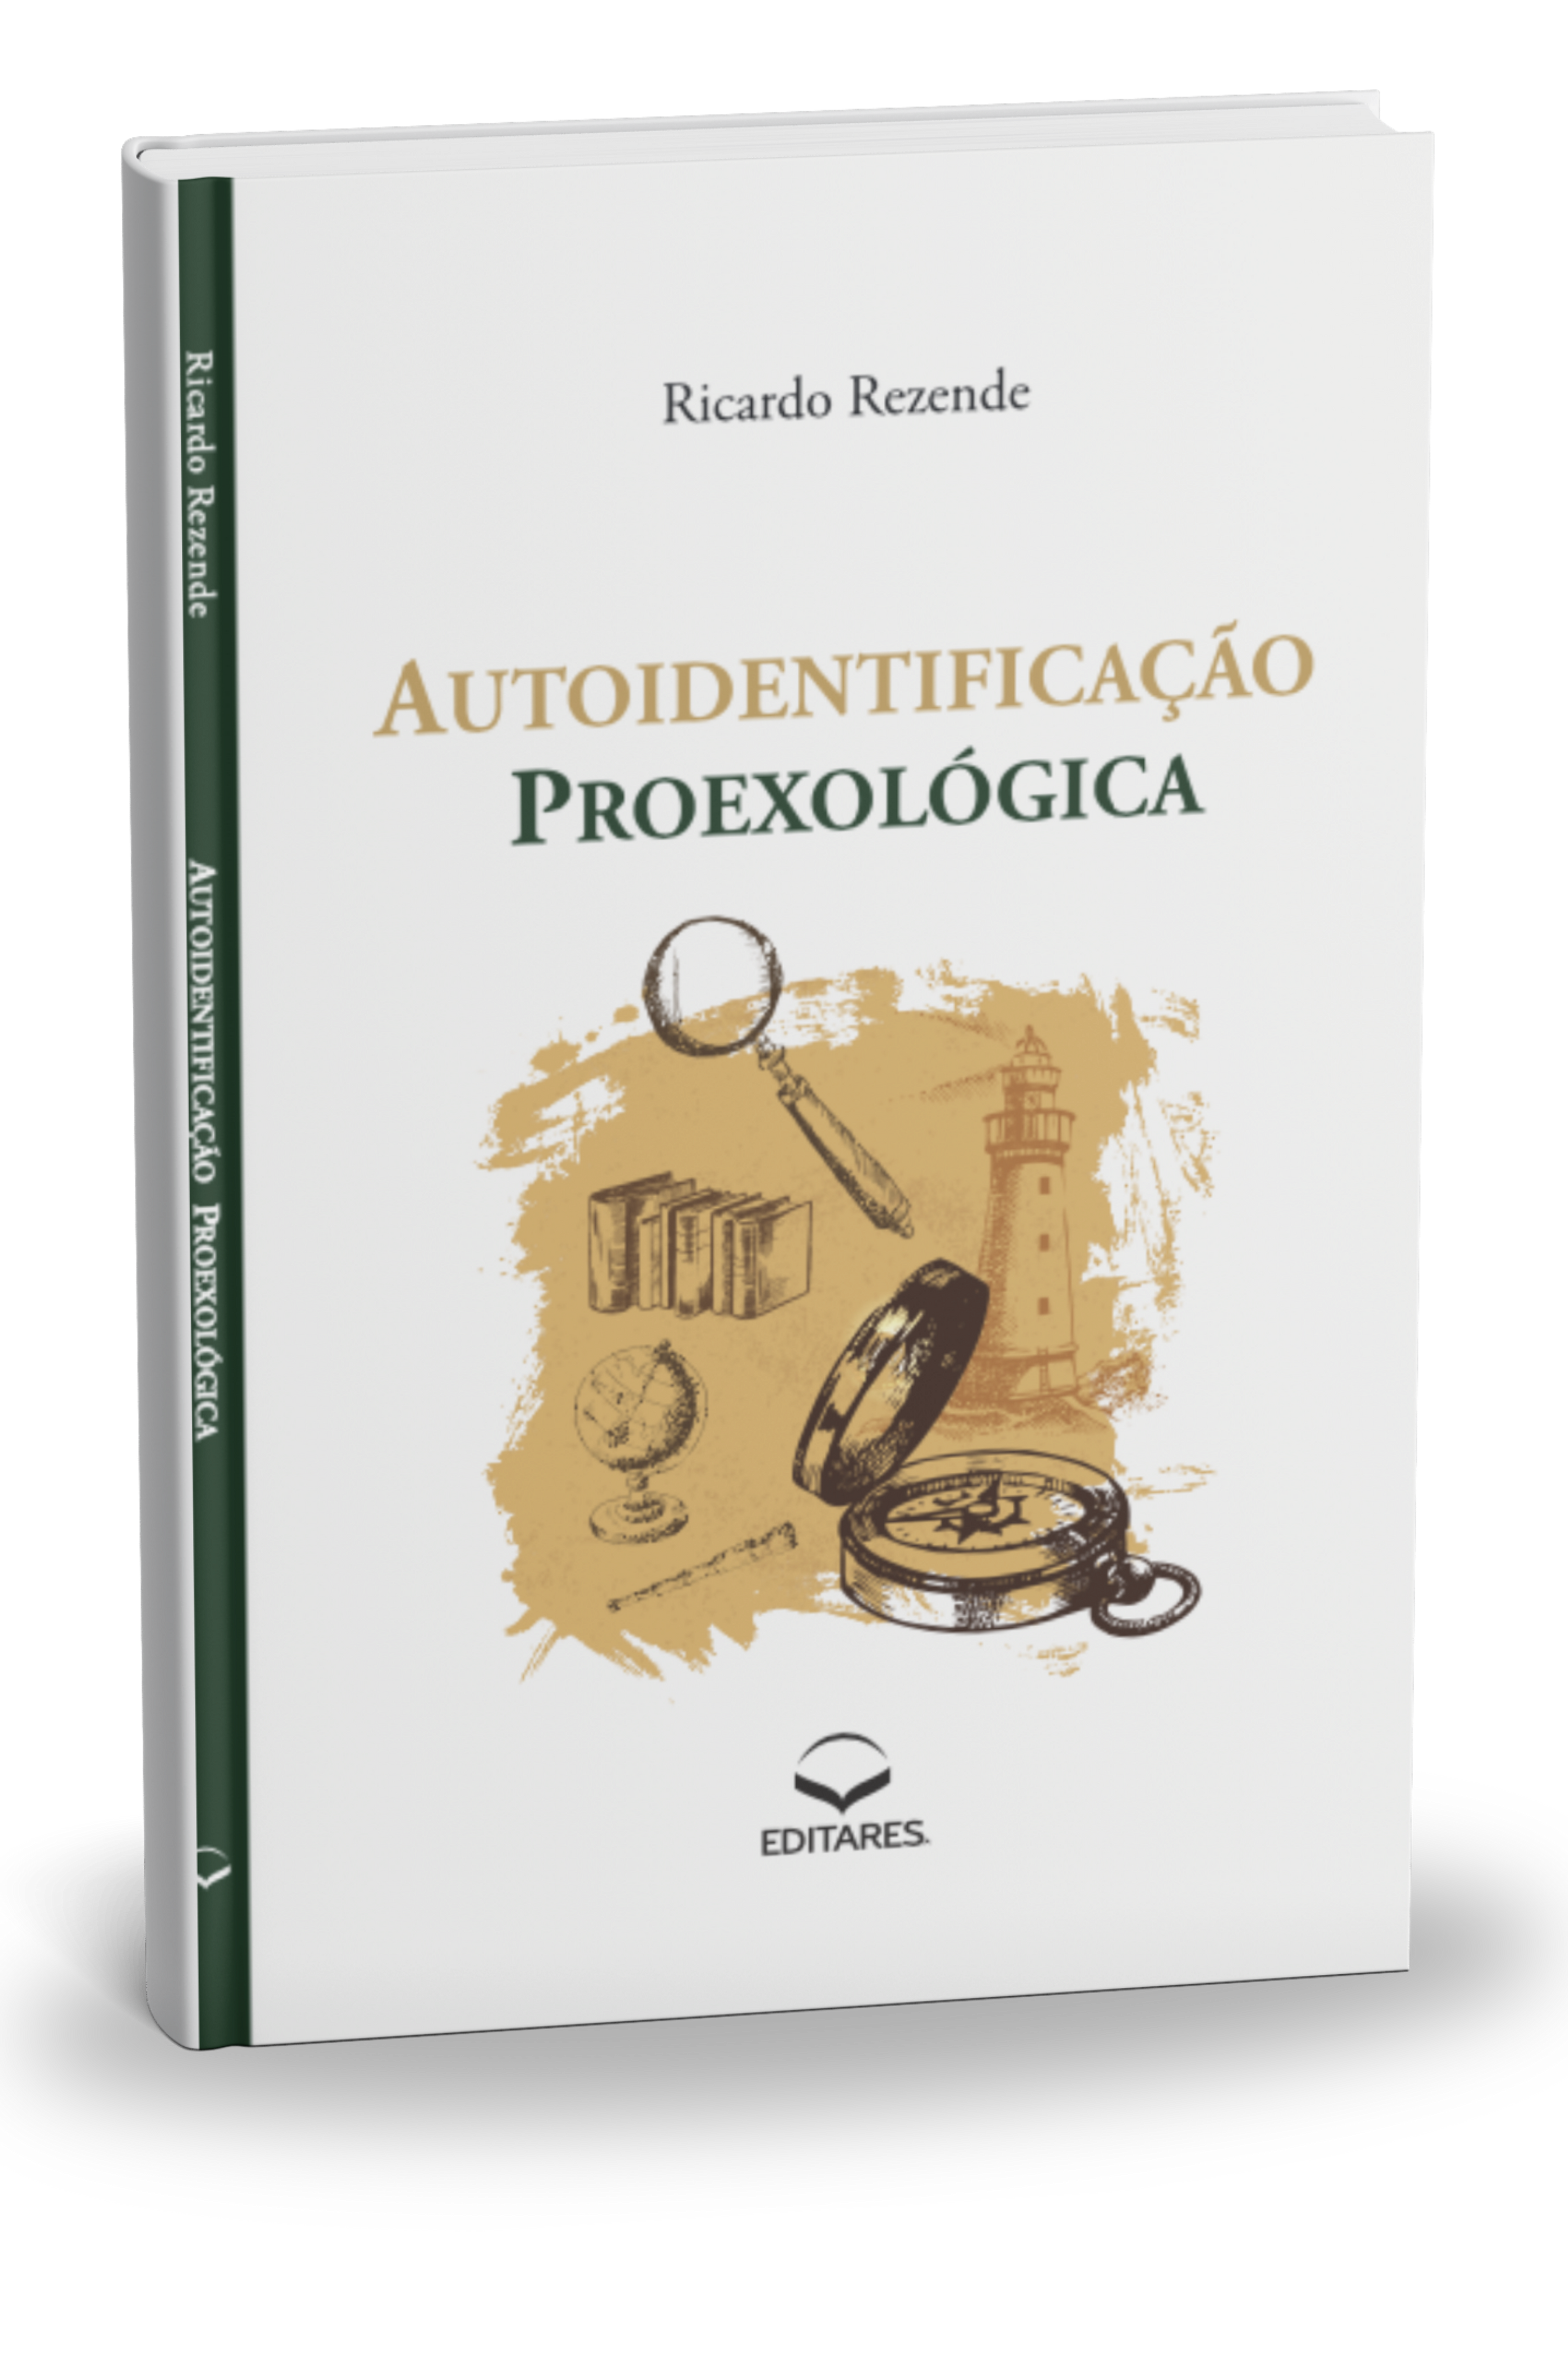
\includegraphics[width=8cm]{articles/entrevista/mockups/Ricardo-Rezende-Proexis.png}
\end{center}

\textbf{1. Qual foi a motivação para a escrita da obra? Por que a definição deste tema para publicação de um livro? }

A ideia de escrever esta obra surgiu em diálogo extrafísico com consciex amparadora, autorrememorada após o despertamento físico. A paraindicação dessa autogescon causou surpresa desconfortável porque não pensava em escrever livro com essa temática e estava priorizando outro trabalho gesconográfico. Apesar disso, desde jovem, confio, coopero com os amparadores extrafísicos e não pretendo mudar esse ortoposicionamento. Assim, acatei a paratarefa.

\begin{pullquote}
    ``A paraindicação dessa autogescon causou surpresa desconfortável porque não pensava em escrever livro nessa temática e estava priorizando outro trabalho gesconográfico''
\end{pullquote}

\textbf{2. Quais foram as principais percepções, intra e extrafísicas, durante a pesquisa e a escrita da obra? }

No decorrer da redação dos capítulos da obra, para a criação dos conteúdos, era necessário rever situações marcantes do próprio passado, ao modo de retrospectivação autobiográfica, relativas às memórias intermissivas e retrovidas pessoais. Nesse processo de revisão e análise de retrofatos particulares, constatava estar juntando, ordenando e encaixando no lugar certo as peças de complexo quebra-cabeças autoconscienciológico, sob os ângulos da \textit{Proexologia, Duplologia, Extrafisicologia, Intermissiologia e Holobiografologia.}

\textbf{3. Qual o maior aprendizado com a escrita desta obra? }

A compreensão aprofundada sobre a identificação e o desenvolvimento da autoproéxis.

\textbf{4. O que poderia dizer como incentivo para que mais pesquisadores invistam na publicação de obras conscienciológicas?}

O hábito da escrita conscienciológica com publicações seriadas resulta na ampliação dinâmica da hiperacuidade e na sustentação da conexão profícua com os amparadores extrafísicos e o holopensene homeostático da autoparaprocedência cursista, favorecendo o desenvolvimento intraconsciencial e da interassistencialidade tarística.

\begin{pullquote}
    ``O hábito da escrita conscienciológica com publicações seriadas resulta na ampliação dinâmica da hiperacuidade e na sustentação da conexão profícua com os amparadores extrafísicos e o holopensene homeostático da autoparaprocedência cursista.''
\end{pullquote}
    
    \end{multicols}
\end{document}


